\section{Workflow for the hybrid-solvent CpHMD in CHARMM} 
As all MD simulations, CpHMD consists of three stages: system preparation, equilibration, and production.
We will explain each stage using a specific protein as an example. 
To follow along, the tutorial files for soluble proteins can be 
downloaded from our GitLab website \href{https://gitlab.com/shenlab-amber-cphmd/cphmd-tutorial/-/tree/main/hphmd_charmm}{cphmd-tutorial/hphmd\_charmm}
and for transmembrane proteins, 
the tutorial files can be downloaded from \href{https://gitlab.com/shenlab-amber-cphmd/cphmd-tutorial/-/tree/main/memb_hphmd_charmm}{cphmd-tutorial/memb\_hphmd\_charmm}.
We will use the pH replica-exchange protocol \cite{Wallace_Shen_2011_J.Chem.TheoryComput.}
in all the examples.

 %--------------------------------------------- 
\begin{figure*}[htb!]
    \centering
    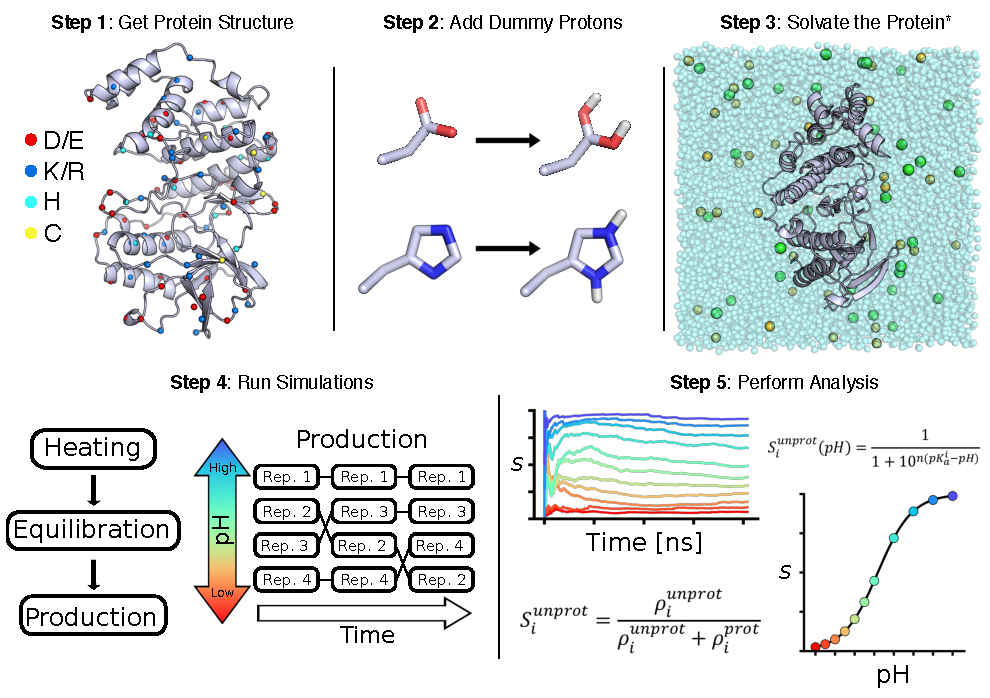
\includegraphics[width=6.6in]{figs/workflow_scheme.pdf}
    \caption{\textbf{Overview of the CpHMD workflow} 
    %Step 5: Add 0 and 1 to the S range.
    %Titration plot, S ==> S_i
    }
    \label{fig:intro}
\end{figure*}
 %--------------------------------------------- 


%------------------------------------------------------------------------------------
\subsection{System Preparation}

To demonstrate CpHMD simulations of 
soluble proteins without retaining the crystal waters,
we use the mini-protein BBL as an example.
The tutorial files for system preparation can be found 
in the directory
\href{https://gitlab.com/shenlab-amber-cphmd/cphmd-tutorial/-/tree/main/hphmd_charmm/bbl_sys_prep}{bbl\_sys\_prep}.

\begin{checklist}{Input files for preparation of a soluble protein}
%\begin{checklist}{Files Produced}
%\textbf{A list of files needed for the equilibration of a soluble protein}
\begin{itemize}
% \item System coordinates (.pdb/.crd)
% \item System topology (.psf)
%%\item Crystal Image Transformations (crystal$\_$image.str)
% \item Periodic boundary conditions (.pbc)
\item step1\_add\_h.inp
\item step2a\_make\_waterbox.inp
\item step2b\_solvate.inp 
\end{itemize}
\end{checklist}

\paragraph{Step 1. Prepare a protein structure with dummy hydrogens.}
First, we retrieve the coordinates of a protein structure
from \href{https://www.rcsb.org/}{Protein Data Bank}\cite{Berman_Bourne_2000_NucleicAcidsRes.},
e.g., BBL (PDB: 1w4h \cite{Ferguson_Fersht_2005_J.Mol.Biol.}).
A homology modeling tool such as SWISS-MODEL\cite{Waterhouse_Schwede_2018_NucleicAcidsRes.} 
can be used to add any missing atomic coordinates.
Next, we convert the PDB file from the standard PDB format to the CHARMM PDB format using the MMTSB tool command \cite{Feig_Brooks_2004_J.Mol.Graph.Model.} \href{http://blue11.bch.msu.edu/mmtsb/convpdb.pl}{convpdb.pl}
or a user supplied script followed by a shell command ``sed'' to
change all histidine residue names to HSP to facilitate titration.

%
\begin{lstlisting}
$ perl convpdb.pl -out charmm22 -segnames
-renumber 1 1w4h.pdb | sed "s/HSD/HSP/g" 
> start.pdb
\end{lstlisting}
%
Here, the output PDB file is formatted for CHARMM (-out charmm22); the segment names are included in the output (-segnames); the residue identification numbers (resid) are renumbered starting at 1; and 
the input file is "1w4h.pdb."
The CHARMM default tautomer for His is HSD.
Changing HSD to HSP indicates to the CpHMD program that histidine is titratable (see later discussion of the parameter file).
Although all resid have been renumbered starting from 1, this does not have to be the case.
Next we add hydrogen atoms to the protein using the HBUILD facility\cite{Brunger_Karplus_1988_Proteins} in CHARMM
\cite{Brooks_Karplus_2009_J.Comput.Chem.}.

To allow titration of Asp and Glu sidechains, we place dummy hydrogens on both carboxylate oxygens.
Note, the dummy atoms do not interact with each other 
and only one is turned on when Asp/Glu is protonated
\cite{Khandogin_Brooks_2005_Biophys.J.}.
The dummy hydrogens are placed in the \textit{syn} position, 
because it is considered
more favorable than the \textit{anti} position
(see discussion in Ref \cite{Khandogin_Brooks_2005_Biophys.J.}).
To prevent the dummy hydrogens from moving to the \textit{anti} position, in which case nonnative hydrogen bonds may form
and a neutral dummy may lose the ability to gain charge,
in the CpHMD specific force field parameter file,
the C--O bond rotation energy barrier
is increased from the standard 0.5 to 6.0 kcal/mol
(see discussion in Ref \cite{Khandogin_Brooks_2005_Biophys.J.}).

Following the addition of hydrogens, a brief energy minimization is performed to correct unfavorable positions.
Here 50 steps of steepest descent (SD) and 10 steps of adopted basis Newton-Raphson (ABNR) are used, whereby a harmonic restraint with the force constant of 50 kcal/mol/{\AA}$^2$ is placed on the heavy atoms.
In most cases the N- and C-terminal ends of the protein are truncated and require capping. 
For N-terminus, we use CH$_3$CO (patch ACE) and 
for C-terminus we use NH$_2$ (patch CT2) or NHCH$_3$ (patch CT3).
In special cases, the free ionized form, NH$_{3}^{+}$ and COO$^+$, is used and can be set titratable when CpHMD is turned on. 
The input file `step1a\_add\_h\_prot.inp' is an example of how to perform these steps on BBL and can be run with the following command.
%
\begin{lstlisting}[language=bash]
$ charmm -i step1a_add_h_prot.inp -o step1a.out
\end{lstlisting}
%
The example input also checks for disulfide bonds using a sulfur-to-sulfur distance cutoff of 2.5 {\AA}. 
After running any input file, make sure to visualize the output 
structure to confirm all the dummy hydrogens and additional features are correctly constructed. 

\paragraph{Step 2. Prepare a solvated system}
Now we move to protein solvation by first building a large 
water box of the desired size.
This is done by generating a plane of small cubic water boxes 
along the x- and y-axes, and then stacking the planar water boxes along the z-axis.
CHARMM toppar directory contains the cubic water box made
of pre-equilibrated TIP3P waters.
The size of the large water box is calculated based on the longest
dimension of the protein and a padding space between the protein 
and the edges of the water box.
We recommend having at least $\sim$10{\AA} padding in x, y, and z directions.
The large cubic water box is then reshaped to a truncated octahedron by removing waters in all eight corners. 
The input file `step2a\_make\_waterbox.inp' is used to construct the octahedron water box.
%
\begin{lstlisting}[language=bash]
$ charmm -i step2_make_waterbox.inp -o 
step2_make_waterbox.out
\end{lstlisting}
%
Once the water box is built, the protein is placed at the center and water molecules within 2.8 {\AA} of the protein heavy atoms are deleted.

The solvated system is subject to energy minimization to release unfavorable contacts. 
First, the protein heavy atoms are fixed and the system undergoes energy minimization using SD and ABNR for 50 steps each. 
Next, a five-stage minimization is conducted with the harmonic constants
of 100, 50, 25, 5, and 0 kcal/mol on the protein heavy atoms using 50 steps of SD and 100 steps of ABNR in each stage. 
The input file
``step3\_solvate.inp'' 
can be used.
%
\begin{lstlisting}[language=bash]
$ charmm -i step2b_solvate.inp -o
step2b_solvate.out
\end{lstlisting}
%
Again, always remember to visualize the system and make sure the system has been constructed to your expectations. 

\subsection{System preparation that includes crystal waters}

\begin{checklist}{Required inputs}
%\begin{checklist}{Files Produced}
%\textbf{A list of files needed for the equilibration of a soluble protein}
\begin{itemize}
% \item System coordinates (.pdb/.crd)
% \item System topology (.psf)
%%\item Crystal Image Transformations (crystal$\_$image.str)
% \item Periodic boundary conditions (.pbc)
\item step1a\_add\_h\_prot.inp
\item step1b\_add\_h\_crys\_wat.inp
\item step1c\_merge\_prot\_crys\_wat.inp
\item step2a\_make\_waterbox\_crys\_wat.inp
\item step2b\_solvate\_crys\_wat.inp 
\end{itemize}
\end{checklist}

In some cases the X-ray structure contains water molecules and it is desirable to keep them, e.g., those in the enzyme active site.
A tutorial showing how to set up a system with crystal waters can be
found in the directory \href{https://gitlab.com/shenlab-amber-cphmd/cphmd-tutorial/-/tree/main/hphmd_charmm/crys_wat_system_prep}{crys\_wat\_system\_prep}.
Here we use a small protein, staphylococcus nuclease (SNase), as an example,
as the X-ray structure (PDBid: 3hzx) contains crystal waters.
% In the previous example, the solution NMR structure of BBL did not contain crystal waters.\cite{Ferguson_JMolBiol_2005_v353_p427}
To keep the crystal waters, just a few additional steps are needed.
First, move all the water molecules into a separate PDB file and make sure the file is properly formatted with the correct column names and column spacing.
In the tutorial the crystal water coordinates have been exported into the the file 'xwat$\_$original.pdb'; however, this file needs to be formatted for use in CHARMM. 
The Python script 'mod$\_$xwat.py' reformats this file, and in the example the reformatted file is named 'xwat$\_$final.pdb', and you might be able to modify the script for your simulation needs.
Most error messages involving the handling of crystal waters are due to the PDB file not being properly formatted. 

Since the crystal waters resolved in a X-ray structure do not contain hydrogen positions, they can be added using the CHARMM input file 'step1b$\_$add$\_$h$\_$xwat.inp'.
With hydrogens added to the protein and crystal waters, the two sets of coordinates need to be combined using the CHARMM input file 'step1c$\_$merge$\_$prot$\_$xwat.inp'.
The rest of the system preparation is very similar to
that without crystal waters.
The only difference to note is when you solvate the system you can merge the segids of the crystal waters (segid: XWAT) with the bulk water (segid: SOLV) using the following command.
%
\begin{lstlisting}[language=bash]
JOIN XWAT SOLV renumber
RENAME SEGID SOLV sele segid XWAT end
\end{lstlisting}
%
Keep in mind this needs to be done after the deletion of water that overlaps with the protein; otherwise you run the risk of accidentally removing some crystal waters.
An example of this is the input file 'step2b$\_$solvate$\_$crys$\_$wat.inp'.


\subsection{System preparation for transmembrane proteins}

\begin{checklist}{Required inputs}
 \begin{itemize}
 \item step1-5/*.inp
  \item step6/*.inp
% \item System Atom Coordinates (.pdb/.crd)
% \item System Atom Topology (.psf)
% \item System Assemtion nbly Info. (.str)
% \item Crystal Image Transformations (crystal$\_$image.str)
% \item Periodic Boundary Conditions (.pbc)
% \item Pre-Equil. System Coordinates (.crd/.pdb)
% \item Pre-Equil. System Trajectory (.dcd)
% \item Pre-Equil. System Information (.out)
% \item Pre-Equil. System Energies (.ene)
% \item Pre-Equil. System Restart (.rst)
\end{itemize}
\end{checklist}
Due to the presence of a lipid bilayer, the preparation of transmembrane proteins for CpHMD simulations requires additional steps.
We divide the preparation into the initial and final stages.
% First, we assemble the system including the protein
% and the solvated lipid bilayer followed by the relaxation of the bilayer. 
The related files can be accessed from the directories
\href{https://gitlab.com/shenlab-amber-cphmd/cphmd-tutorial/-/tree/main/memb_hphmd_charmm/initial_system_prep/}{initial\_system\_prep}
and \href{https://gitlab.com/shenlab-amber-cphmd/cphmd-tutorial/-/tree/main/memb_hphmd_charmm/final_system_prep/}{final\_system\_prep}.

In the initial system preparation, a solvated protein-membrane system is built.
%we first prepare the protein structure using `step1\_genpsf.inp'.
We start by retrieving the protein structure from the database \href{https://opm.phar.umich.edu/}{OPM} (Orientations of Proteins in Membranes), which properly orients the protein in the lipid bilayer using theoretical calculations and experimental data.\cite{Lomize_Mosberg_2006_Bioinformatics}
Just like for soluble proteins, any missing residues need to be added.
%and then the missing hydrogens can be added.
Here we adopt the standard protonation states, i.e., Asp(-), Glu(-), Cys(0), Lys(+), and Arg(+).
As the solution or model {\pka} of His is 6.54 \cite{Thurlkill_Pace_2006_ProteinSci.}, 
which is within one unit of the physiological pH, special attention needs to be given to its protonation (singly or doubly protonated) and tautomeric state (HSD or HSE), based on the nearby hydrogen bonding or salt-bridge interaction. 
% The protonation state of His can be set by changing the residue name in the PDB file and running the script. 
Like soluble proteins, the N- and C-terminal ends may be capped or if necessary the charged forms may be used. 

With the complete protein structure (all heavy atom positions
are in place), we use the script
\href{https://gitlab.com/shenlab-amber-cphmd/cphmd-tutorial/-/tree/main/memb_hphmd_charmm/initial_system_prep/step1-5}{step1\_genpsf.inp} to build
hydrogen positions followed by a short energy minimization in the GB implicit-solvent model to adjust any energetically
unfavorable hydrogen positions.
Next, we build the rest of the system and equilibrate the
lipid bilayer
following the CHARMM-GUI protocol for placing the lipids, solvating the system, and adding ions.\cite{Jo_Im_2007_PLoSONE}
The input files for these steps can be found in the directory \href{https://gitlab.com/shenlab-amber-cphmd/cphmd-tutorial/-/tree/main/memb_hphmd_charmm/initial_system_prep/step1-5}{step1-5}.
Below we will briefly go through the steps.

After the protein structure is prepared, we 
place it at the origin and estimate its 
cross section using the script
\href{https://gitlab.com/shenlab-amber-cphmd/cphmd-tutorial/-/tree/main/memb_hphmd_charmm/initial_system_prep/step1-5}{step2.1$\_$orient.inp}. 
The next step is to add water to the pore of the protein 
using the script \href{https://gitlab.com/shenlab-amber-cphmd/cphmd-tutorial/-/tree/main/memb_hphmd_charmm/initial_system_prep/step1-5}{step2.2$\_$pwat.inp}.
To determine the system dimensions the script \href{https://gitlab.com/shenlab-amber-cphmd/cphmd-tutorial/-/tree/main/memb_hphmd_charmm/initial_system_prep/step1-5}{step3.1$\_$size.inp} is used. This script also assesses the lipid type area and the number of lipids required to be placed between the protein boundary and the periodic boundary condition. 
Approximately 4 to 5 lipids should be placed between the protein and the PBC. 
Additionally, the script will state the thickness of the water slab above and below the lipid bilayer. 
With the dimensions of the system calculated, the lipid heads using big dummy spheres are placed to estimate the positions of the lipids in the bilayer. This is accomplished by \href{https://gitlab.com/shenlab-amber-cphmd/cphmd-tutorial/-/tree/main/memb_hphmd_charmm/initial_system_prep/step1-5}{step3.2$\_$packing.inp}.
Then the dummy spheres are replaced with lipid molecules from a library of randomized conformations using the script \href{https://gitlab.com/shenlab-amber-cphmd/cphmd-tutorial/-/tree/main/memb_hphmd_charmm/initial_system_prep/step1-5}{step4.1$\_$lipid.inp}.
In this example 1-palmitoyl-2-oleoyl-sn-glycero-3-phosphocholine (POPC) lipids are used, but if different lipids are needed other libraries of randomized conformations of lipid molecules can be found on the \href{https://www.charmm-gui.org/?doc=archive&lib=lipid}{CHARMM-GUI Archive - Individual Lipid Molecule Library}.

Next, a rectangular water box is generated using the input file \href{https://gitlab.com/shenlab-amber-cphmd/cphmd-tutorial/-/tree/main/memb_hphmd_charmm/initial_system_prep/step1-5}{step4.2$\_$waterbox.inp}, which solvates the protein and membrane complex.
Next the number of ions required to achieve the desired salt concentration is calculated and randomly placed in the slabs of water above and below the protein and membrane complex. 
In the final step, \href{https://gitlab.com/shenlab-amber-cphmd/cphmd-tutorial/-/tree/main/memb_hphmd_charmm/initial_system_prep/step1-5}{step5$\_$assembly.inp}, all of the system components are combined.
After the system is built, 
all components of the system are relaxed in six equilibration stages with gradually decreased harmonic restraint potentials using the scripts  \href{https://gitlab.com/shenlab-amber-cphmd/cphmd-tutorial/-/tree/main/memb_hphmd_charmm/initial_system_prep/step6}{step6.1$\_$equi.inp to 'step6.6$\_$equi.inp}.

Now we move to the final system preparation stage

%--------------------------------------------------------------------------------
\subsection{Equilibration of soluble proteins}
%--------------------------------------------------------------------------------

\begin{checklist}{Files Required}
%\textbf{A list of files needed for the equilibration of a soluble protein}
\begin{itemize}
% \item System Atom Coordinates (.crd)
% \item System Atom Topology (.psf)
% \item Periodic Boundary Conditions (.pbc)
\item equil\_hphmd.inp
%\item C22 Protein Topologies Parameters (.rtf/.prm)
%\item Water/Ion Topologies and Parameters (toppar$\_$water$\_$ions.str)
%\item C22 Hybrid PHMD Parameters (toppar$\_$phmd$\_$c22.str)
%\item Hybrid PHMD Parameters (phmd$\_$hybrid$\_$g2$\_$c22.in)
%\item GBSW Radii (radius$\_$gbsw.str)
\end{itemize}
\end{checklist}

% \begin{checklist}{Files Produced}
% %\textbf{A list of files needed for the equilibration of a soluble protein}
% \begin{itemize}
% \item Lambda Values (.lamb)
% \item Trajectory (.dcd)
% \item Energy Outputs (.ene)
% \item Restart (.rst)
% \end{itemize}
% \end{checklist}

Equilibration of soluble proteins for CpHMD is performed at a single pH in several stages. 
An example input for the BBL protein is
\href{https://gitlab.com/shenlab-amber-cphmd/cphmd-tutorial/-/tree/main/hphmd_charmm/bbl_equil_prod}{equil\_hphmd.inp}.
% , `\href{https://gitlab.com/shenlab-amber-cphmd/cphmd-tutorial/-/tree/main/hphmd_charmm/bbl_equil_prod}{equilibration$\_$hphmd.inp}.'
Since CpHMD is turned on during equilibration, titratable residues must be chosen. 
In the example here, Asp, Glu, and His are allowed to titrate because of the pH range used in the production simulation.
The crystal structure pH condition or physiological pH 7.4 can be used.
We specify the physiological ionic strength of 0.15 M and temperature of 298 K.
Before invoking the PHMD module for CpHMD
simulation, we need to call GBSW using the following command.
%
\begin{lstlisting}
GBSW HYBRID SGAMMA 0.005 NANG 50 CONC 0.15 - 
SELE protein END
\end{lstlisting}
%
Here, SGAMMA (default 0.005) is the non-polar surface tension coefficient, NANG (default 50) is the number of angular integration points, and CONC (default 0.15) is the ionic strength.
Except for CONC, which the user may change according to the specific problem, the default parameters should be used.

Now we invoke PHMD and set related options using the following command.
%\href{https://hpc.nih.gov/apps/charmm/c42b2html/phmd.html}{PHMD module} to your input file. 
%
\begin{lstlisting}
PHMD PAR 23 WRI 25 PH 7.4 NPRI 5000 PHFRQ 5 
    MASS 10.0 BARR 2.0 BETA 5.0 TEMP 298 LAM -
    SELE RESN ASP .or. RESN GLU .or. RESN HSP end
\end{lstlisting}
%
Here PH is the simulation pH (default 7);
NPRI is the frequency of printing lambda values (5000 means 10 ps);
PHFRQ is the update frequency for the lambda coordinates (default 5);
TEMP is the temperature for $\lambda$ dynamics (default 298);
MASS is the fictitious mass of the $\lambda$ particles (default 10); 
BARR is the quadratic barrier height (default 2.0 and is overwritten by the values specified in the parameter file phmd.inp); 
BETA is the friction coefficient for lambda dynamics (default 5.0); 
LAM tells the PHMD module to output lambda values; and
SELE specifies the types of residues allowed to titrate (default all residues in phmd.inp file). 
Except for PH, NPRI, and SELE options, 
the default settings should be used.

The length of each stage depends on the system and should be adjusted accordingly.
%stages lasting 40 to 120 ps have been used by group for previous projects.
In the BBL example \href{https://gitlab.com/shenlab-amber-cphmd/cphmd-tutorial/-/tree/main/hphmd_charmm/bbl_equil_prod}{equil\_hphmd.inp},
the heating/equilibration stages were run for 20 ps, 
because the system is very small and stable. 
First, the system is heated in the NVT ensemble, and next
% If the system does not require heating the initial and final temperatures can be set to be the same value and the system can equilibrate the water positions under the NVT ensemble.
four stages of equilibration are performed in the NPT ensemble with decreasing harmonic restraints on the heavy atom positions, e.g., 5.0, 1.0, 0.1, and 0 kcal/mol/{\AA}$^2$. 
The idea here is to slowly relax the system by removing any high energy contacts and to allow for the initialization of protonation states at the specified pH (e.g., 7).
% Using four equilibration stages the harmonic constraints on the protein heavy atoms are reduced with the following values 5.0, 1.0, 0.1 (kcal/mol), and then in the last stage all harmonic restraints are released.
% After each equilibration make sure the energies of the system have equilibrated.
Note, the equilibration time for the mini-protein BBL
is short, and you can adjust it accordingly for larger proteins.
%You are now ready to start the production run. 
% The example equilibration input provided moves through each heating/equilibration stage in one input file (equilibration$\_$hphmd.inp). 

\subsection{Equilibration of transmembrane proteins}

\begin{checklist}{Required input files}
\begin{itemize}
% \item  System Atom Coordinates (.crd)
% \item  System Atom Topology (.psf)
% \item  Pre-Equil. System Coordinates (.pdb)
% %\item  Final Lipid Equilibration Snapshot (.pdb)
% \item  Crystal Image Transformations (crystal$\_$image.str)
%\item *.crd, *.psf, 
\item  step0.1$\_$equil.inp
\item  step0.2$\_$equil.inp
\item  step0.3$\_$equil.inp
\end{itemize}
\end{checklist}

% \begin{checklist}{Files Produced}
% \begin{itemize}
% \item Lipid Equilibration Trajectories
% \item CpHMD Trajectory at a Single pH (.dcd)
% \item Lambda Values (.lamb)
% \item Energy Outputs (.ene)
% \item Restart (.rst)
% \end{itemize}
% \end{checklist}

Here, the protein heavy atoms are harmonically restrained using a 1.0 kcal/mol/{\AA}$^2$ until the lipid bilayer is equilibrated in all equilibration simulations.
Starting from the final snap shot of the pre-equilibration simulations ('Pre-Equil. System Coordinates'), the simulation is briefly run for 0.2 ns using an NVT ensemble.
Then a much longer NPT ensemble simulation is run to fully equilibrate the simulation. 
These simulations should be run until the surface area per lipid, bilayer thickness, and lipid order parameters are near or within error limits of experimental lipid composition you are simulating.\cite{Huang_Shen_2021_MethodsinMolecularBiology}
These three lipid bilayer metrics are frequently used to assess the phase behaviour and fine structure of the simulated bilayer.\cite{Klauda_Pastor_2010_J.Phys.Chem.B}
Simulations up to 100 ns can be necessary for proper equilibration of the lipid bilayer.
Since this can be performed on any scalable MD engine we leave this step up to the user to decide which MD engine they would like to use.
For convenience we have supplied \href{}{example input files} for performing this step using the MD software NAMD.\cite{Phillips_Schulten_2005_J.Comput.Chem.}

Following equilibration of the lipid bilayer,
the system can now be equilibrated at a single pH with CpHMD. 
To start this process, dummy protons need to be added in the same manner as for soluble proteins. 
Example input files are in the directory \href{https://gitlab.com/shenlab-amber-cphmd/cphmd-tutorial/-/tree/main/memb_hphmd_charmm/final_system_prep}{final\_system\_prep}. 
%to show how the system is prepared for CpHMD equilibration.
% The first step to break the final snap shot from the lipid equilibration simulation into separate components (Protein, Bilayer, Bulk Water, Pore Water, Sodium Ions, Chloride Ions, ect.).
First, we add hydrogens 
%or the protein all of the hydrogens can be removed and re-added 
with the CHARMM input file 
\href{https://gitlab.com/shenlab-amber-cphmd/cphmd-tutorial/-/tree/main/memb_hphmd_charmm/final_system_prep}{step1a$\_$add$\_$h.inp}.
Next, PSF and CRD files are generated for the rest of the system components with the following scripts
\href{https://gitlab.com/shenlab-amber-cphmd/cphmd-tutorial/-/tree/main/memb_hphmd_charmm/final_system_prep}{step1b$\_$genpsf$\_$memb.inp}, \href{https://gitlab.com/shenlab-amber-cphmd/cphmd-tutorial/-/tree/main/memb_hphmd_charmm/final_system_prep}{step1c$\_$genpsf$\_$water$\_$bulk.inp}, 
\href{https://gitlab.com/shenlab-amber-cphmd/cphmd-tutorial/-/tree/main/memb_hphmd_charmm/final_system_prep}{step1d$\_$genpsf$\_$water$\_$pwat.inp},
\href{https://gitlab.com/shenlab-amber-cphmd/cphmd-tutorial/-/tree/main/memb_hphmd_charmm/final_system_prep}{step1e$\_$genpsf$\_$ion$\_$sod.inp}, and
\href{https://gitlab.com/shenlab-amber-cphmd/cphmd-tutorial/-/tree/main/memb_hphmd_charmm/final_system_prep}{step1f$\_$genpsf$\_$ion$\_$cla.inp}.
Once all the PSF and CRD files have been made,
the rest of the system can be rebuilt using the CHARMM input file 
\href{https://gitlab.com/shenlab-amber-cphmd/cphmd-tutorial/-/tree/main/memb_hphmd_charmm/final_system_prep}{step2$\_$assemble.inp}.

Now three short equilibration steps can be performed using CpHMD at a single pH.
Example inputs are in the directory \href{https://gitlab.com/shenlab-amber-cphmd/cphmd-tutorial/-/tree/main/memb_hphmd_charmm/cphmd_equil}{cphmd\_equil}. 
As for a soluble protein, the specified pH should be the pH used in the crystal growth, physiological pH, or an experimentally relevant pH.
In the first step, the CpHMD simulation is performed 
in the NVT ensemble
with the harmonic force constant of 1.0 kcal/mol/$\mbox{\AA}^2$ for 0.1 ns using the input
\href{https://gitlab.com/shenlab-amber-cphmd/cphmd-tutorial/-/tree/main/memb_hphmd_charmm/cphmd_equil}{step0.1$\_$equil.inp}
In the second step, the CpHMD simulation is performed 
in the NPT ensemble, but the first simulation ('step0.1$\_$equil.inp') uses the NVT ensemble and the second ('step0.2$\_$equil.inp') uses the NPT ensemble.



\href{https://gitlab.com/shenlab-amber-cphmd/cphmd-tutorial/-/tree/main/memb_hphmd_charmm/cphmd_equil}{step0.2$\_$equil.inp}

The third simulation ('step0.3$\_$equil.inp') continues with an NPT ensemble for 0.8 ns with all restraints removed. 
For membrane-enabled CpHMD simulations the tmemb features needs to be added to the \href{https://hpc.nih.gov/apps/charmm/c42b2html/gbsw.html}{GBSW module} in the CHARMM input file. 
%
\begin{lstlisting}
GBSW HYBRID SGAMMA 0.0 NANG 50 CONC 0.15 - 
     TEMP 310 TMEMB 30 MSW 2.5 -
     RCYLN 15 SELE solu END
\end{lstlisting}
%
The inputs variables tmemb, msw, and rcyln are used to build a low dielectric slab to represent the lipid bilayer in the GBSW model with a high dielectric hole centered around the protein.
The TMEMB variable sets the slab thickness ($\mbox{\AA}$) and should be set to the average difference in the $Z$ positions of the lipid C2 atoms from the top and bottom leaflets. This will vary for different lipid types. 
The MSM variable is the half membrane switching length\cite{Im_Brooks_2003_Biophys.J.} for the dielectric transition region between the low-dielectric slab and the bulk solution, and is commonly set to 2.5 $\mbox{\AA}$.
Finally, rcyln is the radius of the high dielectric hole in the low dielectric slab and should set so there is minimal overlap between the protein and lipids.
The protein selection, the last line in the GBSW module, required the protein selection to place the hole at the center of the protein.
Without restraints on the protein heavy atoms, a cylindrical restraint with a harmonic force constant (0.1 kcal mol$^{-1}$ {\AA}$^{-2}$) needs to be applied to the protein to prevent from a lateral drift. 
This can be done using the MMFP facility in CHARMM.

\subsection{Production}

% \begin{checklist}{Files Required}
% \begin{itemize}
% \item System Atom Coordinates (.crd)
% \item System Atom Topologies (.psf)
% \Item Final Equilibration Restart (.rst)
% \item Prod. Input (prod\_hphrex.inp)
% \item Replica Exchange Input (rep.cmd)
% \end{itemize}
% \end{checklist}

\begin{checklist}{Files Produced}
\begin{itemize}
\item CpHMD Trajectories per pH (.dcd)
\item Lambda Values per pH (.lamb)
\item Replica Exchange Info. per pH (.log)
\item Energy Output per pH (.ene)
\item MD Info. per pH (.out)
\item Restarts per pH (.rst)
\end{itemize}
\end{checklist}

The CpHMD production stage is the same for both soluble and transmembrane proteins. 
The only differences are in the set up of the GBSW module to include a low dielectric slab to represent the lipid bilayer for transmembrane simulations, which is discussed in the equilibration stage.
On our GitLab page we have provided examples of the production run for both the \href{https://gitlab.com/shenlab-amber-cphmd/cphmd-tutorial/-/tree/main/hphmd_charmm/bbl_equil_prod}{soluble proteins} and \href{https://gitlab.com/shenlab-amber-cphmd/cphmd-tutorial/-/tree/main/memb_hphmd_charmm/prod}{transmembrane proteins} simulations titled 'production$\_$hphrex.inp' with an example queue submission file for a HPC cluster ('hphrex.qsub').
To begin the production run one must choose a pH range and the number of pH replicas. 
For instance, a protein of interest may be active over a particular pH range or you might want to capture conformational dynamics that include specific titratable residues, such as Asp or His. 
Next you need to decide how many pH replicas to use for your production run. 
Somethings to consider are how many CPUs you have available and how many CPUs you want to allocate to each replica. 
Simulations with CHARMM do not scale well past 8 CPUs, so for a job using 16 replicas you will need 128 CPUs. 
The spacing of the pH replicas needs to be close enough to obtain sufficient exchange probabilities (e.g., 20$\%$).
Typically, to obtain overlap between potential energy distributions of neighboring replicas a pH spacing in increments of 0.25 or 0.5 is required. 
Exchange attempts are made every 1000 steps, and a typical CpHMD simulation of this type will have an average exchange rate of $\sim$40$\%$, if exchange rates are too low more replicas can be added to fill in the spacing between replicas.
To achieve enhanced sampling several replicas should move across all pH replicas.
To use pH-based replica exchange in CHARMM the following \href{https://hpc.nih.gov/apps/charmm/c39b2html/repdstr.html}{REPD} module must be used.
%
\begin{lstlisting}
REPD NREP 8 PHMD EXLM FREQ 5000 UNIT 17
\end{lstlisting}
%
Here, the REPD command initiates replica exchange, NREP states the number of replicas to use, in this case 8, and PHMD states this is pH-based replica exchange and allows for the exchange of $\lambda$ along with the spatial coordinates.
Next, EXLM allows for Hamiltonian exchange and FREQ is how often an exchange is attempted. 
Then to run several replicas in parallel CHARMM reads in a rep.cmd file for each pH replica with the syntax, rep.cmd$\_$0, rep.cmd$\_$1, to rep.cmd$\_$(NREPS), using the following command in the input file.
%
\begin{lstlisting}[language=bash]
$ stream rep.cmd
\end{lstlisting}
% 
Notice this command lacks the '$\_0$' portion of the name.
In each of the rep.cmd file you will have the command that states the pH environment of the replica.
%
\begin{lstlisting}
PHMD RESPH OLDPH @crysph NEWPH @ph PKATEMP @temp
\end{lstlisting}
%
Here OLDPH is the pH used in the equilibration and NEWPH is the pH of the replica.
Finally, PKATEMP should be set to the same temperature of the simulation. 
The rest of the replica exchange set up follows a standard molecular dynamics run in CHARMM.
Production run inputs for BBL (production$\_$hphrex.inp and rep.cmd) can be used to run one 2 ns stage of pH-Replica Exchange CpHMD.

\subsection{General settings for MD and CpHMD in CHARMM}
% CHARMM Specific
% Things to Include: 
%   -) FFs
%   -) Thermostats
%   -) Baristas
%   -) Cutoffs
%   -) ect...

For all simulations the protein 
is represented by CHARMM22/CMAP force field.\cite{MacKerell_Karplus_1998_J.Phys.Chem.B,MacKerell_Brooks_2004_J.Am.Chem.Soc.}
Note, the CpHMD simulations are currently not compatible with the CHARMM36 protein force field.
For solvent the CHARMM modified TIP3P water model is used.
For ions or lipid molecules the CHARMM36 force fields are used.\cite{Klauda_Pastor_2010_J.Phys.Chem.B}
The van der Waals energies are calculated with a switching function from 10 to 12 {\AA} and  a cutoff at 14 {\AA}. 
All simulations are conducted under periodic boundary conditions. 
The PME method\cite{Darden_Pedersen_1993_J.Chem.Phys.} is used to calculate the long-range electrostatic energies and forces with a real space calculation cutoff of 12 {\AA} and 1 {\AA} grid spacing, and a 6th-order spline interpolation. 
The non-bond neighbor list is updated heuristically. 
Additionally, the SHAKE\cite{Ryckaert_Berendsen_1977_J.Comput.Phys.} algorithm is used to constrain all bonds involving hydrogens to allow for a 2-fs time step. 
For NPT simulations, the temperature is maintained with the N\'{o}se-Hoover thermostat.\cite{Nose_Nose_1984_Mol.Phys.,Hoover_Hoover_1985_Phys.Rev.Aa}
The pressure is maintained with the Langevin piston pressure-coupling algorithm.\cite{Feller_Brooks_1995_J.Chem.Phys.}
For CpHMD simulations, the default GBSW radii \cite{Nina_Roux_1997_J.Phys.Chem.B,Chen_Brooks_2006_J.Am.Chem.Soc.} are used for the protein.
For the small molecule, generic atomic radii in the GBSW file may be used upon user verification. 
A CpHMD parameter file phmd.inp contains
the model {\pka} values and deprotonation potential of mean force for the titratable groups Asp, Glu, His, Cys, and Lys. 
Parameters for additional titratable groups
can be obtained by following the steps discussed in section Parameterization.
% As shown in the example inputs the titration ($\lambda$) and tautomer ($\chi$) should be updated every 5 MD steps, allowing for water and lipid relaxation.\cite{Wallace_Shen_2011_J.Chem.TheoryComput.}
% A friction coefficient of 5 ps$^{-1}$ should be used for Langevin dynamics and the mass of the titration coordinate ($\lambda$ and $\chi$) should be 10 atomic mass units. 